\documentclass[a4paper, 12pt]{article}
\usepackage[american]{babel}
\usepackage[utf8]{inputenc}
\usepackage{csquotes}
\usepackage[style=apa,backend=biber,natbib=true]{biblatex}
\DeclareLanguageMapping{american}{american-apa}
\usepackage[T1]{fontenc}
\usepackage{mathptmx}
\usepackage{enumerate}
\usepackage{amsmath}
\usepackage{graphicx}
\usepackage{float}
\usepackage{tikz}
\usepackage{pgfgantt}
\usetikzlibrary{shapes.geometric, arrows}
\usepackage[margin=1.0in]{geometry}

\addbibresource{main.bib}

\renewcommand{\baselinestretch}{1.0}
\newcommand\nd{\textsuperscript{nd}\xspace}
\newcommand\rd{\textsuperscript{rd}\xspace}
\newcommand\nth{\textsuperscript{th}\xspace}

\graphicspath{{./figures/}}
\DeclareGraphicsExtensions{.pdf,.png,.jpeg}

\setlength\parindent{24pt}

% fill up your name, ID, contribution and paper title here
\author{
HAZRIQ ZALFAR BIN HAFIZAL \quad 252UC252WL \quad 100\% \\
}
\title{PASSWORD REUSABILITY : USER BEHAVIOR,
SECURITY RISKS AND MITIGATION
STRATEGIES}
\date{}

\begin{document}
\maketitle

\section*{Abstract}
One of the main problems in modern cybersecurity is still the reuse of passwords. Despite being fully aware of the dangers, users frequently reuse passwords across many platforms in an attempt to prevent mental fatigue. This paper looks at the behavioral aspects that contribute to pass word reusability, the security risks that arise, especially from password stuffing attacks, and the performance of current technical countermeasures. Although user education is still crucial, we think that systemic reforms toward passwordless authentication and automated credential management are required to reduce this danger.

\vspace{0.8cm}

\textbf{Keywords:} Password; Reusability; Authentication, Cybersecurity; Behavior

\newpage

\tableofcontents

\newpage

\section{Introduction}
The key aspect of the problem is the relationship between security and user experience in password systems. It discusses how password standards impact both the degree of protection against cyberattacks and user convenience. The main issue is the trade-off between security and usability. Stronger password requirements, including lengthy, complex passwords that are frequently changed, make users more vulnerable to hacking and phishing attacks. Strict rules, however, often lead to unintended user behavior, such writing down passwords, using them for several accounts, or choosing patterns that are predictable. These weaknesses threaten the exact security that those regulations were meant to protect.
This happened because one of the most frequent attack methods is password leaks.
Even the most advanced protections are useless if users cannot handle their credentials. In addition, its impact on the economy may lead to data breaches that cost companies millions of ringgit in reimbursement, legal liability, and reputational damage. Studying this topic is crucial to responding to evolving cyberthreats and developing policies that improve protection and usability while ensuring user compliance while maintaining security.

\section{Problem Statement}
\subsection*{The Root Problem}
Passwords continue to be the most popular authentication technique, according to studies, but users find it difficult to comply with complicated criteria, which encourages unsafe behaviors like reuse or weak patterns. Strong security regulations and human usability clash, which frequently compromises security. Current strategies, including regular password changes or strict complexity guidelines, have downsides because they irritate users and fail to prevent current threats like phishing or credential stuffing. To ensure that security and usability are balanced, a review of the literature is required to find gaps, assess effectiveness, and investigate new approaches like multi-factor authentication or passwordless systems.

\subsection*{Research Gaps}
Through analyzing multiple research works, several research gaps can be identified: 
\begin{enumerate} 
	\item Small sample numbers and insufficient study verification methods: For instance, Kablo et al. (2024) only spoke with 11 participants when looking at security audit interfaces in password managers. Although their findings provide useful insights into usability and adoption, the small sample limits generalizability and highlights the necessity for larger-scale experimental validation to verify whether these outcomes hold true across broader groups.
 
	\item Restricted geographic scope: Fernando et al. (2023) investigated password usage and security breaches, however they primarily used studies from specific regions, such as Sri Lanka and Europe. Due to the lack of global perspectives in this narrow emphasis, user behaviors and usability difficulties in various cultural and geographic contexts continue to be understudied. Determining the generalizability of findings might benefit from extensive worldwide research.
	
	\item Absence of technique comparisons: Wasfi \& Stone (2023) noted that there isn't a comprehensive side-by-side examination to assess the usability, memorability, and attack resistance of textual, passphrase, mnemonic, and recognition-based password schemes. Without such comparison studies, it is difficult to identify which approaches provide the best security and usability balance for different user groups.
\end{enumerate}


\section{Research Questions, Hypotheses and Objectives}
\subsection*{Research Questions}
\begin{enumerate}
	\item What approaches have been used by researchers to improve password usability while maintaining strong security?

    \item What are the major findings reported in existing studies regarding user behavior and password management?

    \item What limitations exist in current password usability approaches, and how do they affect overall cybersecurity?

    \item What research gaps and future opportunities can be identified to design more effective and user-friendly authentication systems?
\end{enumerate}

\subsection*{Hypotheses}
\begin{enumerate}
	\item H1: Approaches that integrate password managers and multi-factor authentication significantly improve usability while maintaining strong security compared to traditional password-only systems.
 
    \item H2: Users tend to prioritize convenience over security, leading to widespread password reuse and weak password choices, despite awareness of cybersecurity risks.

    \item H3: Current usability-focused password policies, such as frequent mandatory changes, complex composition rules, inadvertently increase password reuse and reduce memorability, thereby weakening overall cybersecurity.
    
    \item H4: Incorporating explainable password audit tools and adaptive authentication mechanisms will reduce password reuse and improve user trust, addressing gaps in current usability-focused approaches.

\end{enumerate}

\subsection*{Objectives}
\begin{enumerate}
	\item To evaluate the extent of password reuse across multiple accounts among different demographic groups within six months.
    
    \item To analyze the impact of password reuse on overall system vulnerability by simulating attack scenarios within a controlled environment.

    \item To compare the effectiveness of password managers versus manual password strategies in reducing reuse over a three-month experimental period.
    
    \item To identify usability limitations in current password policies that encourage reuse and propose improvements within one year.

\end{enumerate}

\section{Literature Review Summary}
This review's goal was to examine password usability with a particular focus on the relationship between security procedures and user behavior. The primary findings show that, although identification-based methods and password managers offer some solutions, memorability, storage practices, and password reuse remain significant issues. Significant research limitations include a lack of long-term usability studies, a limited number of different user samples, and the insufficient examination of hybrid or passwordless systems. The general conclusion is that current approaches are insufficient to achieve a balance between security and usability, despite developments. Future research alternatives include developing flexible and user-friendly authentication methods, looking into hybrid models, and implementing passwordless technologies to address unresolved usability difficulties.

\section{Research Methodology}

\subsection{Research Design}
The research will use a mixed-methods approach that combines simulation-based modeling, quasi-experimental comparisons, and empirical surveys. While controlled tests will contrast the use of password managers with manual methods, surveys will record user behavior and demographic influences on password reuse. Breach probability under various reuse circumstances will be modeled using Monte Carlo simulations. This design ensures quantitative validation of security threats as well as qualitative insights into user behavior.

\subsection{Technical Approach}

\begin{enumerate}
    \item Monte Carlo Simulation : Used to estimate breach likelihood when reused passwords are exposed in large datasets.

    \item Comparative Framework : Two user groups, password manager users and non-users, will be studied to measure differences in password uniqueness and strength.

    \item Algorithm Development : Prototype an explainable password audit tool that provides transparent feedback on password weaknesses.

    \item Usability Testing : Apply heuristic evaluation and task-based testing to identify limitations in password creation policies and their effect on reuse.

\end{enumerate}

\subsection{Data and Tools}
\begin{itemize}
    \item Statistical Packages: SPSS, Python for quantitative analysis and modeling.
    \item Password Managers: Bitwarden, KeePass, LastPass for experimental comparison between manager users and non-users.
    \item Simulation Frameworks: MATLAB, Python (NumPy/SimPy) for Monte Carlo modeling and probabilistic simulations.
    
\end{itemize}


\subsection{Evaluation Criteria}

\begin{itemize}
    \item Security Metrics: Password entropy, uniqueness, and resistance to dictionary/brute-force attacks.
    \item Usability Metrics: Task completion time, error rates, memorability, and user satisfaction scores.
    \item Performance Metrics: Simulation accuracy, computational efficiency, and scalability of algorithms.
    \item Adoption Metrics: Percentage of participants reducing reuse after exposure to password managers or audit tools.
    \item Explainability Metrics: User comprehension of audit feedback, measured through post-task questionnaires.
\end{itemize}

\section{Expected Outcomes}
The results of this study should demonstrate that password reuse is still common among a variety of user demographics, primarily due to usability issues and mental limitations. The study will probably reveal that reused passwords greatly enhance vulnerability to widespread breaches by examining survey data and simulation results. It is anticipated that comparative studies will show that password managers, when paired with credential audit tools, boost password uniqueness and decrease reuse in comparison to manual methods. By offering empirical proof of the usefulness of supporting tools in reducing insecure user behaviors, these findings will advance the discipline.

\par These results are important because they increase our knowledge of password usability in both academic and practical contexts. A comprehensive dataset on password reuse trends, a comparative assessment approach for password managers, and a prototype explainable audit tool that boosts user trust by offering clear feedback are among the outputs. Together, these results will influence cybersecurity policy, direct the creation of user-friendly authentication systems, and create new possibilities for the integration of security technology with usability-focused methodologies. Thus, this study will close the gap between theoretical password security models and actual user behavior.

\newpage

\section{Research Activities and Milestones}

\subsection{Research Activities Flowchart}


\usetikzlibrary{shapes.geometric, positioning}

\begin{center}
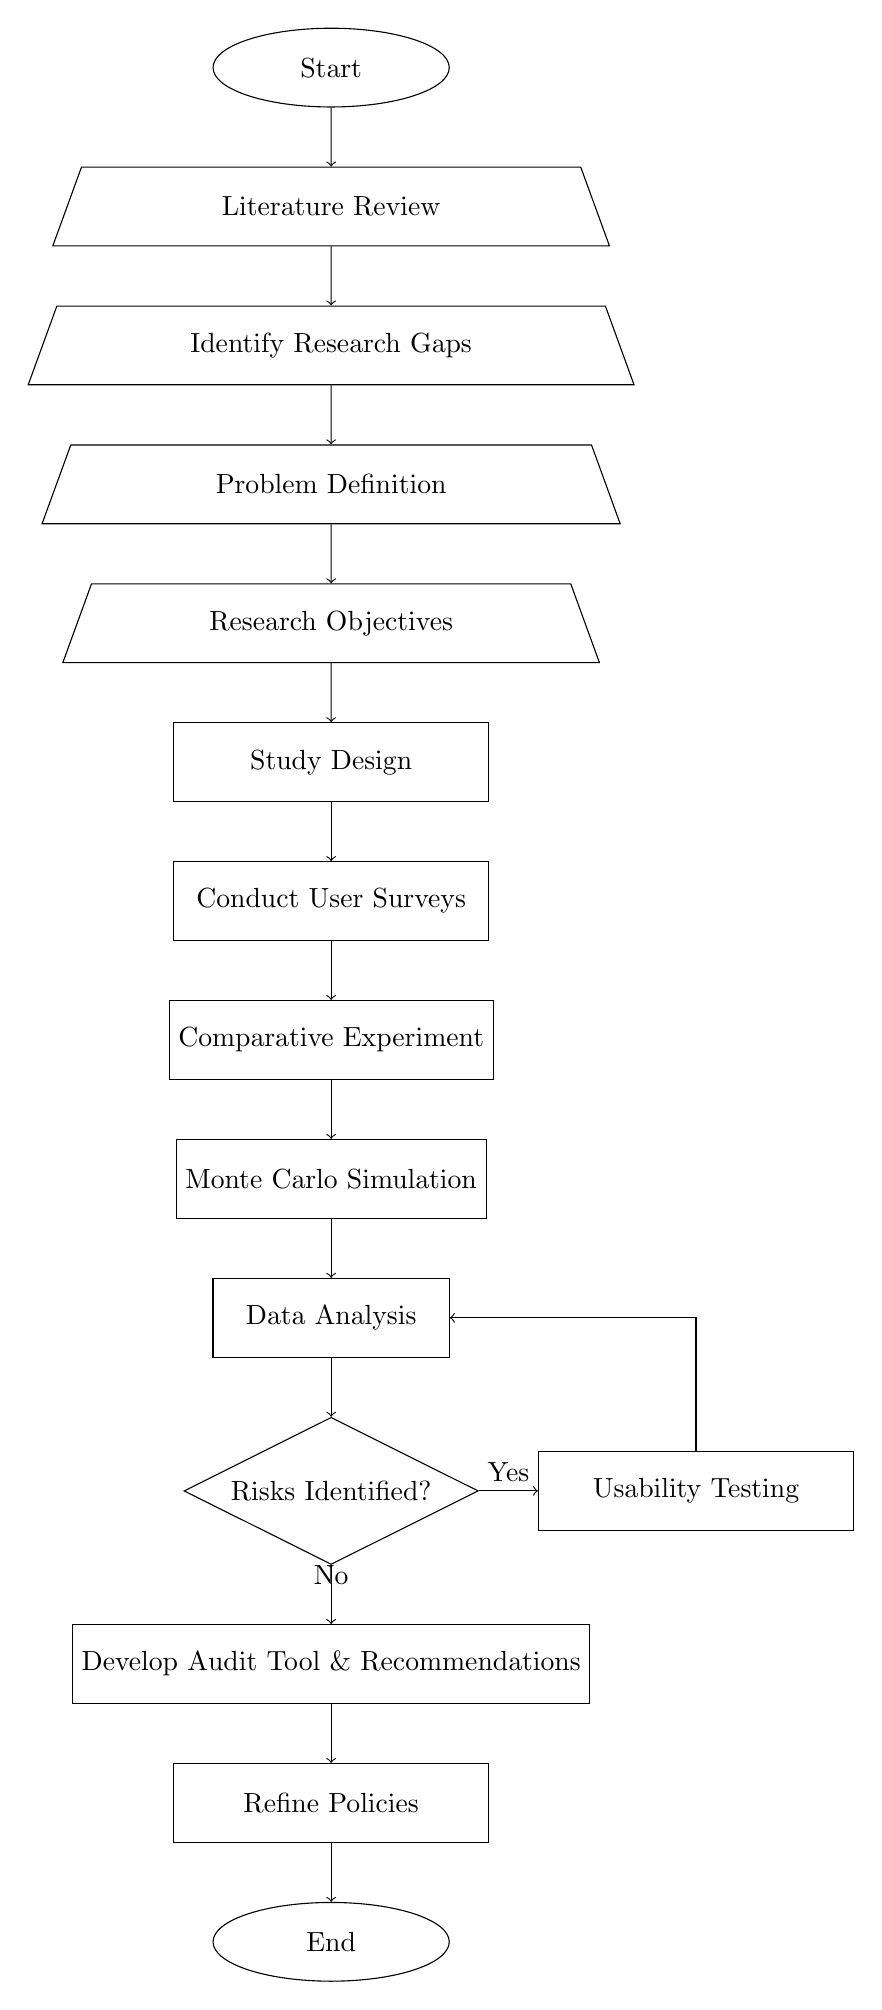
\begin{tikzpicture}[node distance=0.75cm]

    % Start
    \node (start) [ellipse, draw, minimum width=3cm, minimum height=1cm] {Start};

    % Literature Review
    \node (literature) [trapezium, draw, trapezium angle=70, below=of start, minimum width=4cm, minimum height=1cm] {Literature Review};

    % Research Gaps
    \node (gaps) [trapezium, draw, trapezium angle=70, below=of literature, minimum width=4cm, minimum height=1cm] {Identify Research Gaps};

    % Problem Definition
    \node (problem) [trapezium, draw, trapezium angle=70, below=of gaps, minimum width=4cm, minimum height=1cm] {Problem Definition};

    % Objectives
    \node (objectives) [trapezium, draw, trapezium angle=70, below=of problem, minimum width=4cm, minimum height=1cm] {Research Objectives};

    % Study Design
    \node (design) [rectangle, draw, below=of objectives, minimum width=4cm, minimum height=1cm] {Study Design};

    % User Surveys
    \node (survey) [rectangle, draw, below=of design, minimum width=4cm, minimum height=1cm] {Conduct User Surveys};

    % Comparative Experiment
    \node (experiment) [rectangle, draw, below=of survey, minimum width=4cm, minimum height=1cm] {Comparative Experiment};

    % Monte Carlo Simulation
    \node (simulation) [rectangle, draw, aspect=2, below=of experiment, minimum width=3cm, minimum height=1cm] {Monte Carlo Simulation};

    
    % Data Analysis
    \node (analysis) [rectangle, draw, aspect=2, below=of simulation, minimum width=3cm, minimum height=1cm] {Data Analysis};

    % Decision
    \node (decision) [diamond, draw, aspect=2, below=of analysis, minimum width=3cm, minimum height=1cm] {Risks Identified?};

    % Usability Testing
    \node (usability) [rectangle, draw, right=of decision, minimum width=4cm, minimum height=1cm] {Usability Testing};

    % Develop Audit Tool
    \node (audit) [rectangle, draw, below=of decision, minimum width=4cm, minimum height=1cm] {Develop Audit Tool \& Recommendations};

    % Refine Policies
    \node (policy) [rectangle, draw, below=of audit, minimum width=4cm, minimum height=1cm] {Refine Policies};

    % End
    \node (end) [ellipse, draw, below=of policy, minimum width=3cm, minimum height=1cm] {End};

% Arrows
\draw[->] (start) -- (literature);
\draw[->] (literature) -- (gaps);
\draw[->] (gaps) -- (problem);
\draw[->] (problem) -- (objectives);
\draw[->] (objectives) -- (design);
\draw[->] (design) -- (survey);
\draw[->] (survey) -- (experiment);
\draw[->] (experiment) -- (simulation);
\draw[->] (simulation) -- (analysis);
\draw[->] (analysis) -- (decision);

% Branch arrows
\draw[->] (decision.east) -- (usability.west) node[midway, above] {Yes};
\draw[->] (decision.south) -- (audit.north) node[midway, above] {No};
\draw[->] (usability.north) |- (analysis.east);

% Connect branches back to End
\draw[->] (audit) -- (policy);
\draw[->] (policy) -- (end);

\end{tikzpicture}
\end{center}

\newpage

\subsection{Research Activities Gantt Table}
\begin{ganttchart}[
    hgrid,
    vgrid,
    bar height=0.6,
    bar/.append style={fill=blue!50},
    group/.append style={fill=purple!30},
    milestone/.append style={fill=red!70},
    x unit=0.35cm, % scale horizontally
    y unit chart=0.7cm % scale vertically
]{1}{24} % 24 weeks ~ 6 months

% Labels for weeks
\gantttitle{Project Timeline (6 Months)}{24} \\
\gantttitlelist{1,...,24}{1} \\

% Tasks
\ganttbar{Literature Review \& Problem Definition}{1}{4} \\

\ganttbar{Research Design \& Data Collection}{5}{8} \\

\ganttbar{Experimental Implementation \& Simulation}{9}{16} \\

\ganttbar{Analysis \& Evaluation}{17}{20} \\

\ganttbar{Reporting \& Dissemination}{21}{24} \\

\end{ganttchart}

% =========================================
% REFERENCES
% =========================================

\newpage
\section*{References}
\addcontentsline{toc}{section}{References}

%\printbibliography

Kablo, E., Kader, K., \& Arias-Cabarcos, P. (2024, May). " I'm actually going to go and change these passwords": Analyzing the Usability of Credential Audit Interfaces in Password Managers. In Extended Abstracts of the CHI Conference on Human Factors in Computing Systems (pp. 1-13). 
https://dl.acm.org/doi/abs/10.1145/3613905.3650889

\vspace{0.4cm}

Wasfi, H., \& Stone, R. (2023). Usability and security of knowledge-based authentication systems: a state-of-the-art review. 
https://dr.lib.iastate.edu/entities/publication/6e52e358-5352-4b97-93e3-0804fd224d09

\vspace{0.4cm}

Fernando, W. P. K., Dissanayake, D. A. N. P., Dushmantha, S. G. V. D., Liyanage, D. L. C. P., \& Karunatilake, C. (2023). Challenges and opportunities in password management: a review of current solutions. Sri Lanka Journal of Social Sciences and Humanities, 3(2). 
https://account.sljssh.sljol.info/index.php/sljo-j-sljssh/article/view/96

%References
\printbibliography

\end{document}